\chapter{Diseño e implementación}
\label{cap:Diseno}

El presente capítulo detalla la fase de diseño construcción de la aplicación se señalan las decisiones tomadas a lo largo del desarrollo para cumplir con lo solicitado, descrito en el capítulo anterior.

Yendo desde lo general a lo particular se comienza presentando la arquitectura del sistema, construida a partir de los requerimientos establecidos en el capítulo anterior, posteriormente se continúa con las decisiones que llevaron al sistema a ser lo que es.

\section{Arquitectura del sistema}
\label{sec:Arquitectura}

El sistema de detección de necesidades, en su conjunto, consta de dos módulos independientes: el \textit{front-end}, dedicado a la interacción con el usuario, presentación de la información, etcétera; y el \textit{back-end}, orientado a las tareas de procesamiento \textit{online} de los datos para su posterior despliegue.

La comunicación entre los módulos se realiza por medio del almacenamiento de documentos en la base de datos. Esta arquitectura se presenta en la Figura \ref{fig:arquitecturaSistema}. A continuación se detalla cada uno de los elementos que la componen.

\begin{figure}[H]
	\centering
	\captionsetup{justification=centering}
	\includegraphics[scale=0.6]{images/arquitectura.png}
	\caption[Arquitectura del sistema.]{Arquitectura del sistema.\\Fuente: Elaboración Propia, (2016)}
	\label{fig:arquitecturaSistema}
\end{figure}

\subsection{\textit{Back-end}}
\label{subsec:backend}

El módulo de \textit{back-end} corresponde al sistema de detección en sí, todo el sistema está alimentado por el \textit{stream} entregado por la API de \textit{Twitter}, pues en esta red social se generan más de 140 millones de \textit{tweets} diariamente, \cite{StormIBM}, y se dispara en periodos de crisis, \cite{TaxonomiaChato}, por ello es una buena fuente de información primaria, es decir, que viene desde la misma población afectada. Haciendo uso de esta fuente de información da soporte a la historia de usuario HU-c02, que explicita el uso de ésta.

Para el procesamiento de de los datos, que llegan de forma continua se hace uso de \textit{Apache Storm} para construir un grado de procesamiento \textit{ad-hoc} a la aplicación, capaz de filtrar todos los eventos que respondan a los requerimientos de la aplicación. Para ello se utilizan los elementos de \textit{Storm} presentados en la sección \ref{arte:SPS}, \textit{spout} y \textit{bolt} para la construcción de operadores que realicen las tareas necesarias para la transformación de datos. Uno de estos operadores tiene que ver con cómo son compartidos los datos, en este caso, se hace uso de una base de datos no relacional, MongoDB, para compartir datos entre módulos para permitir una comunicación bidireccional, tanto de consultas como de elementos a ser desplegados en la visualización. Otro de los operadores tiene que ver con el etiquetado de datos, para ello se hace uso de un clasificador, almacenado como un archivo, generado haciendo uso de Mallet, \cite{Mallet}, para etiquetar las nuevas entradas como elementos de una categoría en particular. El cómo funcionan éstos operadores se detalla a lo largo de éste capítulo.

Los elementos cuya comunicación se señala con una flecha roja son elementos que están considerados en la arquitectura final, pero que están fuera de los alcances de éste proyecto, ellos son: el sistema detector de eventos que, al detectar que se produce un evento catastrófico en el país, comienza a ejecutar el detector de necesidades; y el módulo etiquetador que recibe un archivo con entradas y las etiqueta para, posteriormente, realizar el entrenamiento de un nuevo clasificador.

\subsection{\textit{Front-end}}
\label{subsec:front}

El módulo correspondiente a la visualización está encargado de desplegar la interfaz de usuario al sistema por medio de su navegador \textit{web}. Hace uso de la información registrada por el módulo de detección de necesidades, la cual es almacenado en la base de datos, para mostrarla al usuario. Para realizar ésto se utilizan las API de Google Maps y Highcharts para, respectivamente, desplegar el mapa geográfico, donde la información es mostrada como marcadores adaptados para cada categoría presente en la aplicación y permita manipular la información de tal forma que se cumpla con lo solicitado por la historia de usuario HU-v02, HU-v03, HU-v06 y HU-v07, y el uso de la línea temporal e histograma de frecuencias utilizados para cumplir con la historia de usuario HU-v04.

Además ésta aplicación proporciona el medio para que el usuario realice consultas al sistema para realizar un filtrado de datos que cumpla con sus necesidades, cumpliendo así con la historia de usuario HU-v05. De igual manera permite el establecimiento de parámetros para el funcionamiento de la aplicación como se especificó en la historia HU-v08.

\section{Características del sistema}
\label{sec:caracteristicasSistema}

A continuación se realiza mencionan las características que ha de tener el sistema, se hace esto para tener en cuenta en las decisiones tomadas en las siguientes secciones.

En primer lugar, es necesario hacer hincapié en el contexto en que el sistema opera. \textit{Twitter} es un servicio que cuenta con millones de usuarios activos, los que generan constantemente nuevo contenido que recuperado por la API de \textit{streaming}. Dado la masividad de los datos generados, se requiere de una plataforma de procesamiento capaz de lidiar con dicha carga y mantener tiempos de procesamiento razonables.

En segundo, y como se explicó en la sección \ref{subsec:HerrDesarrollo}, el funcionamiento interno de las aplicaciones construidas con \textit{storm} se puede esquematizar por medio de un grafo dirigido donde los nodos se corresponden con los operadores definidos en la topología y que pueden tener diferente cantidad de elementos por procesar y tardar tiempos distintos en realizar su labor. Lo anterior sugiere que pueden existir niveles en los que se producen cuellos de botella en el \textit{pipeline} de procesamiento. Considerando lo anteriormente expuesto el sistema ha de estar preparado para responder de la mejor forma posible cuando se produzcan estas obstrucciones en el proceso.

En tercer lugar, el uso de un clasificador de texto involucra que la calidad del etiquetado está dada por el cómo éste se construyó. La construcción está dada por los datos de entrenamiento; mientras más datos se entreguen, probablemente, la calidad del clasificador sea mayor. Esto quiere decir que el clasificador puede ser mejorado y que consituye una limitante el mantener éste estático.

\section{Decisiones de diseño}
\label{sec:decDiseno}

Esta sección presenta las decisiones tomadas por el autor al momento de diseñar las aplicaciones que componen el sistema de detección de necesidades.

\subsection{Comunicación}
\label{sec:diseno:comunicacion}

Se ha de justificar lo expuesto hasta ahora al hacer mención de la existencia de dos módulos que componen el sistema de detección de necesidades. El uso del sistema de procesamiento distribuido, \textit{storm}, dificultaba en su momento la integración con un \textit{framework} para aplicaciones Java y, dado que el sistema ha de poseer una interfáz donde el usuario pueda visualizar los eventos detectados, por ello se decidió construir ambos módulos; detección y visualización de manera separada. En un primer momento se pensó comunicar ambas aplicaciones por medio de peticiones REST cuyo contenido fuesen tanto las consultas ingresadas por el usuario para realizar una búsqueda más exhaustiva, como los datos correspondientes a marcadores ubicados en el mapa del visualizador, pero ésta aproximación no consideraba la existencia de un sistema de persistencia de información; al considerarla, la comunicación ya no se realiza por medio de peticiones REST, sino que se utiliza la base de datos como intermediario. La Figura \ref{fig:comunFinal} presenta cómo se produce la comunicación en el sistema.

\begin{figure}[H]
	\centering
	\captionsetup{justification=centering}
	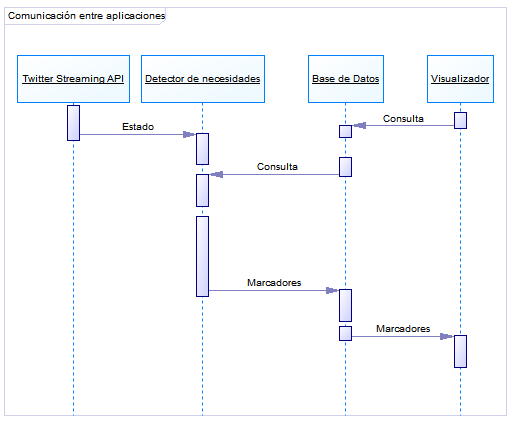
\includegraphics[scale=0.8]{images/ComunicacionFinal.png}
	\caption[Esquema que representa la comunicación entre aplicaciones del sistema detector de necesidades.]{Esquema que representa la comunicación entre aplicaciones del sistema detector de necesidades.\\Fuente: Elaboración Propia, (2016)}
	\label{fig:comunFinal}
\end{figure}

El módulo de detección comienza a alimentarse del \textit{stream} de \textit{Twitter}, a la vez consulta a la base de datos por si se han ingresado nuevas consultas por el usuario. Al obtener la respuesta la utiliza para generar nuevos marcadores los que pasan a ser almacenados en la base de datos, desde donde son obtenidos por la el módulo de visualización para desplegar la información por pantalla.


\subsection{Persistencia}
\label{sec:diseno:persistencia}

Si bien está decidida la implementación de un sistema de persistencia en la aplicación, no se ha definido cuál ha de ser el sistema de gestión de base de datos que se ha de utilizar, es por ello que en ésta sección se presenta la decisión tomada con respecto a este tema.

Debido a que se requiere mantener una ventana de datos históricos se requiere de un mecanismo de persistencia o base de dato. Los datos han de ser almacenados, al menos durante un tiempo, para que el sistema pueda realizar inferencias de información considerando los datos recibidos. 

Se consideraron los principales sistemas de bases de datos utilizados y conocidos por el autor, dentro de los cuales se encontraban herramientas relacionales como: MySQL, PostgreSQL, SQL Server y MongoDB para el caso de sistemas de gestión de base de datos (DBMS) no relacionales. Dadas las características y las condiciones con las cuales opera el sistema de detección se requiere de un DBMS con rápido tiempo de respuesta en operaciones lectura/escritura; la decisión se tomó en base a los datos que se manejaran, pues no se apreció necesidad de implementar una modelo relacional, pues no habían datos que requirieran mantener la consistencia entre relaciones y, es más, se requiere, sobre todo, de rapidez. De esta forma y teniendo en cuenta los resultados presentados en pruebas empíricas realizadas por \cite{MongoPerformance} en las cuales mostró que el tiempo de respuesta (en operaciones de lectura) es significativamente menor en MongoDB que en dos de los DBMS más conocidos como MySQL y PostgreSQL. Lo anterior, sumado al hecho de la capacidad de escalar de MongoDB reportada en fuentes oficiales o por diversos desarrolladores como \cite{MongoDBScalability} que han compartido sus experiencias en la \textit{web}, llevaron a decidir que MongoDB debiera ser el sistema de gestión de base de datos que se utilizase en el sistema.

Para realizar la conexión de MongoDB y el \textit{framework} se utiliza, específicamente, dos bibliotecas: La primera corresponde a un ORM (Mapeo Objeto-Relacional), denominado Jongo, la cual hace uso de la segunda llamada Jackson, para realizar la conversion de JSON a objeto.

Volviendo a la historia de usuario que originó la necesidad de contar con un sistema de persistencia de datos, habiendo resuelto lo anterior la siguiente problemática se presenta como ¿qué datos han de guardarse? Según la definición de la historia en la que se señalan "eventos pasados dentro de un intervalo de tiempo", se infiere que ha de guardarse tanto el contenido visible del dato, la clasificación que se le asignó y la fecha en que se identificó, para ello y dado que se seleccionó MongoDB, se especificó un esquema para los documentos de la colección, dados los datos que se almacenan sólo resta tener la información correspondiente a la ubicación, por lo que el esquema se definió como se presenta en la Figura \ref{fig:esquemaMarker1} correspondiente a la colección "Markers".

\begin{figure}[H]
	\centering
	\captionsetup{justification=centering}
	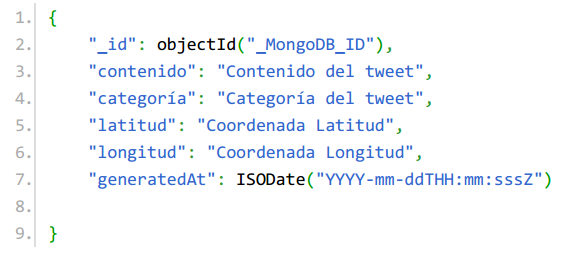
\includegraphics[scale=0.8]{images/Marker1.png}
	\caption[Ejemplo de documento en la colección Markers.]{Ejemplo de documento en la colección Markers.\\Fuente: Elaboración Propia, (2016)}
	\label{fig:esquemaMarker1}
\end{figure}

El primer campo corresponde al ID asignado por mongo para cumplir con la unicidad de los datos, el segundo campo corresponde al contenido textual del \textit{tweet} para ser mostrado junto con el marcador y que el usuario pueda ver desde dónde el sistema asignó aquel \textit{tweet} a una categoría en particular. El tercer campo corresponde al nombre de la etiqueta o categoría asignada al \textit{tweet}, esta asignación está dada por el resultado de la evaluación del clasificador. Los campos cuarto y quinto corresponden a la ubicación geográfica en la que se posiciona el marcador y, finalmente, el sexto campo corresponde al momento en que fue creado el marcador para ser utilizado en los diferentes criterios de visualización del sistema.

\subsection{Sistema de procesamiento}
\label{sec:diseno:sistDeProce}

Ya se mencionó que se seleccionó storm para construir el detector de necesidades, pero no se ha especificado el porqué de ello. Por este motivo en los siguientes párrafos se exponen las razones por las cuales se tomó esta decisión.

Dado el contexto del funcionamiento del sistema, éste ha de entregar respuestas rápidas ante una emergencia; para ello, y como es descrito en la historia de usuario HU-c00, se requiere de un sistema capaz de procesar eventos en tiempo real que, dado la masividad de datos con los que debe lidiar la aplicación, ésta ha de poder escalar. El problema en este punto es el cómo construir un sistema que cumpla capaz de identificar necesidades y que posea esta, no menor, característica.

Se consideraron sistemas de procesamiento distribuido; estos sistemas tienen la particularidad de ser una red de computadores (nodos, en general), que el usuario percibe como un solo gran sistema. Estos sistemas pueden ser de diversos tamaños, y suelen ser confiables, pues en caso de que un componente (nodo) falle, otro es capaz de reemplazarlo. \cite{DefSPD}. En un inicio se consideraron tres plataformas sobre las cuales puede construirse un sistema que pudiese cumplir con lo solicitado; dichas plataformas fueron Apache S4, Apache Storm y Apache Spark.

Apache S4, pese a su simplicidad, no continuó con su desarrollo luego del año 2013 y nunca tuvo una versión estable 1.0, razones por las cuales se dejó como segunda opción. Apache Spark, pese a contar con continuos \textit{releases}, una comunidad de desarrolladores no menor y permitir la elaboración de sistemas escalables no era lo que se buscaba en aquel momento como herramienta de desarrollo, pues está orientado al procesamiento por lotes y no en tiempo real. Al momento de consultar con los, en este caso, clientes, éstos esperaban que el sistema, internamente, se comportara según el paradigma de procesamiento de \textit{streams}, por medio de operadores dispuestos en un grafo. Por ello finalmente se optó por \textit{Apache Storm}.

\textit{Storm} permite construir sistemas que cumplan con las características de un sistema distribuido, como lo son: Escalabilidad (Tanto horizontal como vertical) y tolerancia a fallos (como la capacidad de un sistema para realizar correctamente y en todo momento aquello para lo que fue diseñado). Estos sistemas están compuestos por dos tipos de elementos: \textit{Spout} y \textit{Bolt}, que fueron descritos en el capítulo \ref{cap:MarcTeorico}. Al combinar esos elementos se da origen a un grafo dirigido, como el presentado en la Figura \ref{fig:stormBeLike} en la página ~\pageref{fig:stormBeLike}, donde cada elemento de procesamiento (\textit{bolt}), cumple con una determinada tarea utilizando como entrada la salida del elemento anterior.

\subsection{Fuente de datos}
\label{sec:diseno:obtenerDatos}

La historia de usuaio HU-c01 refleja desde dondé se han de obtener los datos, pero es necesario especificar más aún. Como se señaló al momento de definir los alcances de este trabajo, sólo se utiliza \textit{Twitter} como fuente de información, así la unidad de información pasa, desde ahora, a llamarse como se habitúa en aquella red social: el \textit{Tweet}.

Existen tres tipos de \textit{streaming endpoints} disponibles, cada uno para un caso de uso particular y son descritos en la Tabla \ref{tab:StreamingEndpoints}.

\begin{table}[H]
\centering
\caption[\textit{Streaming endpoints} de \textit{Twitter}.]{\textit{Streaming endpoints} de \textit{Twitter}.\\Fuente: Elaboración Propia, (2016)}
\label{tab:StreamingEndpoints}
\begin{tabular}{|l|l|}
\hline
Público & \begin{tabular}[c]{@{}l@{}}Stream del que fluye la información pública de Twitter.\\ Casos de uso: Seguimiento de usuarios o tópicos específicos o minería de datos.\end{tabular} \\ \hline
Usuario & Flujo que toda la información correspondiente a un usuario.                                                                                                                       \\ \hline
Sitio   & Versión multi-usuario de la anterior.                                                                                                                                             \\ \hline
\end{tabular}
\end{table}

Para esta aplicación la adecuada corresponde a la API pública. En ésta, a la vez, existen dos puntos de acceso; el público y \textit{firehose}. El acceso público es gratuito y permite el acceso a un 1\% de la información que se genera en tiempo real y para acceder a el basta con crear una aplicación dentro de \textit{Twitter}. En cambio para acceder a \textit{firehose}, el cual permite acceso total a la información, debe comprarse el acceso. Dadas estas condiciones se seleccionó, previo acuerdo con los clientes, el uso de la API pública.

Para hacer uso de la API descrita con anterioridad es necesario obtener cuatro claves de acceso: \textit{Access Token}, \textit{Access Token Secret}, \textit{Consumer Key (API Key)} y \textit{Consumer Secret (API Secret)}. Para más información sobre cómo conseguir estas claves consulte el Apéndice \ref{apendice:clavesApi}.

\subsection{Términos de búsqueda}
\label{sec:diseno:termBusqueda}

\textit{Twitter4J}, es una herramienta que permite obtener el flujo de información desde \textit{Twitter} implementa una forma de filtrado mediante el uso de palabras clave, pero posee una limitante al momento de modificar la búsqueda, deben instanciarse nuevamente los objetos con los cuales se realiza la conexión a la API de \textit{Twitter}, eso se traduce en tiempo de procesamiento perdido. Para solucionar este inconveniente se decidió implementar un operador, descrito en la sección \ref{subsec:detectorNecesidades}, el cual está encargado de realizar el filtrado de acuerdo a términos y llevar a cabo la operaciones descritas en la sección \ref{subsubsec:2op} referente a la expansión de la consulta. Sin embargo, un operador como este puede poseer réplicas que operan al mismo tiempo, con esto surge el problema de ¿Cómo comunicar y aplicar los nuevos términos de búsqueda, desechando los antiguos?.

Para dar solución a esta problemática se decidió recurrir a la base de datos; almacenar la consulta y asignar un estado para controlar el comportamiento del operador. Así el esquema en la base de datos queda tal y como se presenta en la Figura \ref{fig:esquemaQuery}, documento de la colección "Queries".

\begin{figure}[H]
	\centering
	\captionsetup{justification=centering}
	\includegraphics[scale=0.8]{images/Query.png}
	\caption[Ejemplo de documento en la colección queries.]{Ejemplo de documento en la colección queries.\\Fuente: Elaboración Propia, (2016)}
	\label{fig:esquemaQuery}
\end{figure}

Donde la propiedad "estado" puede tomar dos valores: "actual" o "antiguo", reflejan si una consulta se está llevando a cabo o no. Estos valores son asignados por la aplicación responsable de la interfaz la responsable de recibir los términos de búsqueda por parte del usuario.

Para implementar este operador se utilizaron dos clases llamadas \textit{CurrentQueryChecker} y \textit{QueryExpander} desarrolladas, la primera, para detectar cuándo y si es que ha cambiado una consulta en la base de datos y la segunda para desarrollar la labor descrita por el algoritmo de expansión descrito en la sección \ref{subsubsec:2op}.

\subsection{Categorización de necesidades}
\label{sec:diseno:categorias}

La definición de las categorías es un punto importante dentro de la construcción de la aplicación. Teóricamente en función a la cantidad de clases (categorías), el tamaño del conjunto de entrenamiento ha de ser mayor o menor.

Inicialmente se consideró la taxonomía definida por \cite{TaxonomiaChato}, pero el equipo del proyecto FONDEF IDeA estableció que no era conveniente utilizar, pues presentaba gran cantidad de categorías y era demasiado específica. Como alternativa se sugirió en su lugar utilizar la clasificación realizada por \cite{PMIProfes}, en la que se presentaba una categorización de cinco categorías. Éstas fueron realizadas por parte de un equipo de psicólogos experos en el contexto del proyecto PMI-USA 1204, basándose en la información obtenida del terremoto de febrero de 2010 y los \textit{twees} recolectados en dicho evento, éstas eran:

\begin{enumerate}
\item Necesidades básicas: \textit{Tweet} que entrege o solicite información sobre serviciós básicos: Agua potable, electricidad y abastecimiento de alimentos.
\item Comunicación: \textit{Tweet} que entregue o solicite información sobre alguna localidad.
\item Seguridad: \textit{Tweet} que señale un riesgo para la población.
\item Personas: \textit{Tweet} que haga referencia al hallazgo o búsquead de una persona desaparecida.
\item Irrelevante: Cualquier otro \textit{tweet}.
\end{enumerate}

Acordando con el equipo, se decidió separar el primer ítem en los tres elementos que lo componen: Agua, alimentos y electricidad. Así, finalmente, se obtienen siete categorías de clasificación.\\

Los elementos clasificados como "Irrelevantes" no se muestran en el mapa de eventos, pues hacen referencia a eventos que, pese a haber pasado por todos los operadores anteriormente descritos, no guardan relación con el evento o sus consecuencias. Éstos pueden ser \textit{tweets} a etiquetar por expertos \textit{a posteriori} con el objetivo de enriquecer la información del clasificador. Esta tarea, sin embargo, está fuera del alcance de este proyecto.

\subsection{Clasificador}
\label{sec:diseno:clasificador}

Se busca generar un clasificador automático capaz de detectar necesidades y lidiar con la jerga nacional. Para ello, según lo descrito por \cite{IRQE} en su libro \textit{Introduction to Information Retrival}, se entrenó un clasificador basado en \textit{Naïve Bayes}, haciendo uso de Mallet, pues en pruebas realizadas con las RapidMiner y Weka, mencionadas en la sección \ref{subsubsec:Classifiers}, alcanzó mejores resultados.

La sección \ref{sec:caracteristicasSistema} ya hace referencia a la inconveniencia de utilizar un clasificador estático para el etiquetado de nuevos eventos, al tratarse de un aprendizaje supervisado, donde se requiere de una persona entregue la respuesta esperada para realizar el entrenamiento, no es posible realizar este proceso de manera automática.

Al no poder automatizar el proceso antes señalado se consultó con el equipo del proyecto FONDEF IDeA si es que era factible la implementación de un actualizador manual del clasificador, lo cual fue aceptado.

Segun la metodologia KDD, los pasos que se siguen para construir un nuevo clasificador son los siguientes:

Los datos son seleccionados por el usuario, estos datos se agruparan en un archivo de texto, un archivo CSV en el cual los elementos se separaran utilizando el caracter punto y coma (;). El formato que se utiliza para el archivo de entrada se muetra en la Figura \ref{fig:formatoFig} , así cualquier archivo que cumpla con el formato permite la creación de un nuevo modelo clasificador.

\begin{figure}[H]
	\centering
	\captionsetup{justification=centering}
	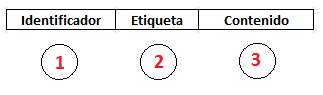
\includegraphics[scale=0.8]{images/FormatoArchivoEntrada.png}
	\caption[Formato archivo de entrada.]{Formato archivo de entrada.\\Fuente: Elaboración Propia, (2016)}
	\label{fig:formatoFig}
\end{figure}

\begin{enumerate}
\item Corresponde a un identificador arbitrario, pero necesario para la herramienta de clasificación Mallet.
\item Corresponde a la etiqueta que categoriza al contenido.
\item Contenido del \textit{tweet} propiamente tal.
\end{enumerate}

El preprocesamiento y transformación de los datos está dado por la definición de los operadores presentados en la sección \ref{subsec:detectorNecesidades}.

Teniendo en consideración que se utilizan dos aplicaciones distintas, donde en una se construye el clasificador y en otra donde es utilizado. Surge el problema de cómo realizar la comunicación entre ellas. Para solucionar este inconveniente se utiliza una carpeta compartida por ambas aplicaciones. En el caso de sistemas Unix se utiliza el directorio $/opt/DeNe$, mientras que para Windows se utiliza $C:/DeNe/$. En estos directorios se almacena un fichero con el clasificador serializado.

\begin{figure}[H]
	\centering
	\captionsetup{justification=centering}
	
\includegraphics[scale=0.8]{images/ClasifierDene.png}
	\caption[Fichero clasificador en $c:/DeNe/$.]{Fichero clasificador en $C:/DeNe/$.\\Fuente: Elaboración Propia, (2016)}
	\label{fig:TopologiaGeneral}
\end{figure}

Cada vez que se actualice el clasificador se contrasta el nuevo con el ya existente, de encontrar mayor precisión en el primero, se reemplaza en la carpeta antes mencionada, según el sistema operativo de la máquina que se esté utilizando. En caso contrario, se mantiene al anterior. En ambos escenarios se le da a conocer al usuario la precisión de ambos.

\subsection{Interfaz web}
\label{sec:diseno:interfaz}

Teniendo en consideración la característica del desarrollo de esta aplicación como un proyecto ágil con un mínimo de personal para desarrollar se requería de un \textit{framework} que contribuyera a acelerar la construcción de la aplicación. Tras considerar las alternativas más conocidas como \textit{Spring}, \textit{Hibernate} o \textit{JSF} que tienen una curva de aprendizaje elevada, se optó por utilizar un cuarto \textit{framework} que aunque desconocido, promete una simplicidad en su uso. \textit{Play Framework}, construido haciendo uso de Scala y Java permite construir aplicaciones ligeras (tamaño en disco), sin estado (no guarda configuraciones de una sesión para ser utilizadas luego) y por defecto RESTful, ideal para la comunicación entre aplicaciones. Éste \textit{framework} sigue el patrón de arquitectura Modelo-vista-controlador (MVC). Cuenta con un compilador en tiempo real (compila y realiza el despliegue de la aplicación cuando detecta un cambio en el código), lo que agiliza en gran medida el desarrollo, pues al automatizar este proceso mantiene la atención en lo que se está desarrollando.

Para visualizar los puntos encontrados por el detector de necesidades se decidió utilizar la API de \textit{Google Maps} la que permite la colocación de los denominados 'marcadores' en un punto específico del mapa y asociar a ellos algún tipo de información. Así, aunque el funcionamiento interno esté dirigido por \textit{Play}, la principal funcionalidad del sistema, mostrar el mapa con sus marcadores, es implementada utilizando Javascript.

Estos marcadores, ya ubicados en el mapa, tienen asociado un cuadro de texto dentro del cual refleja el la categoría a la que pertenece y el \textit{tweet} original, el texto, que lo generó, la Figura \ref{fig:EjemploMarker} presenta un ejemplo del funcionamiento de ésto en la interfaz \textit{web}. Esto tiene como objetivo permitir decidir, en última instancia, al usuario si ha sido correctamente clasificado.

\begin{figure}[H]
	\centering
	\captionsetup{justification=centering}
	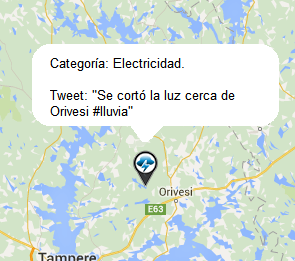
\includegraphics[scale=0.8]{images/EjemploMarker.png}
	\caption[Ejemplo de marcador en el mapa con su categorización y \textit{tweet} que lo generó.]{Ejemplo de marcador en el mapa con su categorización y \textit{tweet} que lo generó.\\Fuente: Elaboración Propia, (2016)}
	\label{fig:EjemploMarker}
\end{figure}

Según lo solicitado en la historia de usuario HU-v02 se prepararon dos tipos de filtros a la interfaz para la visualización de eventos en el mapa: El primero considera el agrupamiento o \textit{clustering} de marcadores, mientras que el segundo considera el tipo de marcador o marcadores que se desean visualizar.

Para el caso del agrupamiento se definieron tres modos de funcionamiento las cuales se describen a continuación:

\begin{enumerate}
\item No agrupar: Mostrar todos los marcadores que correspondan en el mapa de acuerdo al punto geográfico que corresponda en su definición.
\item Agrupar por distancia: Define una grilla invisible en el mapa donde los elementos que calcen en una cudrícula son agregados a un \textit{cluster} y visualizados como tal.
\item Agrupar por categoría: De igual forma que el agrupamiento por distancia, pero sólo agrega elementos que comparan categoría.
\end{enumerate}

Las Figuras \ref{fig:clusterdistancia} y \ref{fig:clustercategoria} presentan un ejemplo de ambos tipos de agrupamiento especial, respectivamente por distancia y categoría.

\begin{figure}[!htb]
	\minipage{0.48\textwidth}
	\centering
	\captionsetup{justification=centering}
	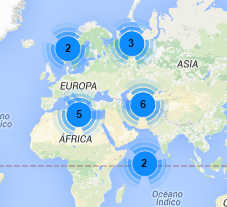
\includegraphics[scale=1]{images/EjemploCluster.png}
	\caption[Ejemplo de agrupamiento basado en la distancia de los marcadores.]{Ejemplo de agrupamiento basado en la distancia de los marcadores.\\Fuente: Elaboración Propia, (2016)}
	\label{fig:clusterdistancia}
	\endminipage\hfill
	\minipage{0.48\textwidth}
	\centering
	\captionsetup{justification=centering}
	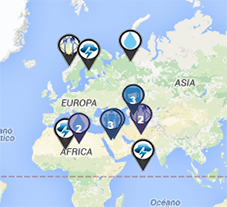
\includegraphics[scale=1]{images/ClusterCategoria.png}
	\caption[Ejemplo de agrupamiento basado en la categorías de los marcadores.]{Ejemplo de agrupamiento basado en la categorías de los marcadores.\\Fuente: Elaboración Propia, (2016)}
	\label{fig:clustercategoria}
	\endminipage\hfill
\end{figure}

Para el segundo caso sólo se definieron dos reglas de funcionamiento las cuales se describen a continuación:

\begin{enumerate}
\item Mostrar todos: Muestra elementos de todas las categorias existentes.
\item Mostrar categoría: Para cada categoría mostrar sólo los elementos de aquella categoría. 
\end{enumerate}

Al combinar ambos tipos de filtros se tienen potencialmente seis modos de funcionamiento, pero considerando las categorías descritas en al sección \ref{sec:diseno:categorias} ese número se expande a veintiún modos de funcionamiento del visualizador.

\section{Implementación del sistema}
\label{sec:implementacion}

Ésta sección detalla las particularidades de presentadas en la implementación de ambos sistemas, tanto del detector de sistema, como del visualizador.

\subsection{Visualizador}
\label{subsec:imp:visualizador}

La implementación del visualizador de eventos se realizó haciendo uso del \textit{framework} de Java \textit{Play}, éste \textit{framework}, por defecto, crea aplicaciones que siguen el patrón de diseño MVC, por lo tanto se tienen tres niveles dentro de la aplicación:

\begin{itemize}
\item Modelo: donde están los elementos que permiten interactual con la base de datos. 
\item Controlador: presentando los métodos de reacción ante los eventos detonados en el nivel de presentación.
\item Vista o presentación: muestra las interfaces \textit{web} diseñadas para que el usuario interactúe con el sistema.
\end{itemize}

\subsubsection*{Filtrado de marcadores}
\label{subsubsec:filtradoMarcadores}

Dentro del nivel de presentación se encuentra el mapa, proporcionado por la API de Google Maps como se mencionó en la sección \ref{sec:diseno:interfaz}. Allí, también, se señaló que existen filtros para la visualización de eventos de manera que se la presentación de éstos se apegue a las necesidades del usuario. Para implementar estos filtros, internamente, la aplicación hace uso de $n + 1$ \textit{clusters}, donde $n$ corresponde al al número de categorías y el cluster extra es para agruparlos a todos. Así, en el caso de querer ver los eventos agrupados, y dependiendo si se quiere o no agruparlos sin discriminación de categoría, se llenan los \textit{clusters} pertenecientes a la visualización general o a la visualización por categoría. Para el caso de querer mostrar sólo una categoría en particular, sólo se permite que los \textit{cluster} se llenen con los elementos de la categoría seleccionada.

Lo anteriormente descrito es presentado a continuación en el Algoritmo \ref{alg:filtroMarcadores} para facilitar la comprensión de la lógica interna de los filtros presentados.\\

\begin{algorithm}[!htb]\setstretch{1.5}
	\begin{algorithmic}[numeracion_lineas]
		\REQUIRE Tipo de agrupamiento $A$.
		\REQUIRE Discriminador de categoría $K$.
		\REQUIRE Marcadores $M$.
		\STATE Lista de marcadores $L$.
		\STATE \textit{Clusters} de marcadores $C = \{c_{0}, \dots, c_{n+1} \}$.
		\FOR{cada $m_{i}$ perteneciente a $M$}
			\IF{la categoría de $m_{i}$ no es "irrelevante" y la categoría de $m_{i}$ es igual a $K$}
				\STATE añadir el marcador a $L$.
			\ELSIF{$K$ es "todas las categorías"}
				\STATE añadir el marcador a $L$.
			\ENDIF
		\ENDFOR
		\IF{$A$ es "no agrupar"}
			\FOR{cada $l_{i}$ perteneciente a $L$}
				\STATE posicionar $l_{i}$ en el mapa.
			\ENDFOR
		\ELSIF{$A$ es "agrupar todos"}
			\FOR{cada $l_{i}$ perteneciente a $L$}
				\STATE añadir $l_{i}$ al clister $c_{0}$.
			\ENDFOR
			\STATE posicionar $c_{0}$ en el mapa.
		\ELSE
			\FOR{cada $l_{i}$ perteneciente a $L$}
				\STATE añadir $l_{i}$ al cluster $c_{i+1}$
			\ENDFOR
			\FOR{cada $c_{i}$ perteneciente a $C - \{c_{0}\}$}
				\STATE añadir $l_{i}$ al cluster $c_{i}$
			\ENDFOR
		\ENDIF
	\end{algorithmic}
	\caption{Algoritmos de utilización de filtros}
	\label{alg:filtroMarcadores}
\end{algorithm}\vphantom\\

Para realizar la selección del intervalo mencionado en la HU-v04 se solicitó, por parte del equipo FONDEF IDeA, el uso de una línea de tiempo con intervalo deslizante que, además, mostrase la cantidad de eventos detectados por fecha por medio de un histograma. Para ello se utilizó, inicialmente, se utilizó \textit{JDateRangeSlider}, de la biblioteca Javascript JQRangeSlider, \cite{JQRangeSlider}. Ésta biblioteca era suficiente para seleccionar el intervalo de fechas y detectar cambios producidos en la línea de tiempo para actualizar los valores, mas no permite la implementación de un histograma externo.

\begin{figure}[H]
	\centering
	\captionsetup{justification=centering}
	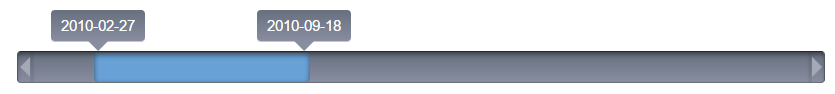
\includegraphics[scale=0.6]{images/JDateRangeSlider.png}
	\caption[Selectorde fechas JDateRangeSlider.]{Selectorde fechas JDateRangeSlider.\\Fuente: \cite{JQRangeSlider}}
	\label{fig:JQRangeSlider}
\end{figure}

Para lograr implementar ambas dos se utilizó una biblioteca Javascript distinta. La Figura \ref{fig:HistogramaFinal} presenta la implementación utilizando \textit{HighCharts}, \cite{Highcharts}. Ésta, al contrario de la anterior, no permitía capturar los cambios en el histograma, para solucionarlo se implementó una función javascript que recogiese los valores del intervalo y arroja un evento cuando se produjece un cambio, este evento se asoció al eje x de la linea temporal, cambiando el valor de la variable \textit{valuesOfAxis} cada vez que se moviese el eje, éste evento es descrito en la Figura \ref{fig:implementacionCambiosEnEje}.

Inicialmente este histograma sólo está disponible en inglés, pero permite cambiar todas sus etiquetas manualmente, así, buscando la usabilidad de la aplicación, se modificaron todos los textos y el resultado está visible en la Figura \ref{fig:HistogramaFinal}.

\begin{figure}[H]
	\centering
	\captionsetup{justification=centering}
	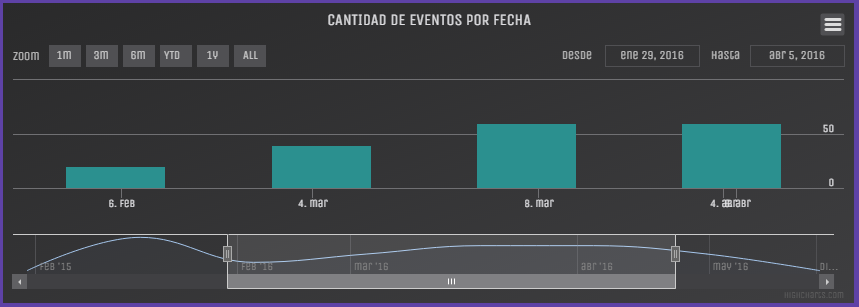
\includegraphics[scale=0.6]{images/Histograma.png}
	\caption[Selector de fechas presente en la aplicación.]{Selector de fechas presente en la aplicación.\\Fuente: Elaboración Propia, (2016)}
	\label{fig:HistogramaFinal}
\end{figure}

\begin{figure}[H]
	\centering
	\captionsetup{justification=centering}
	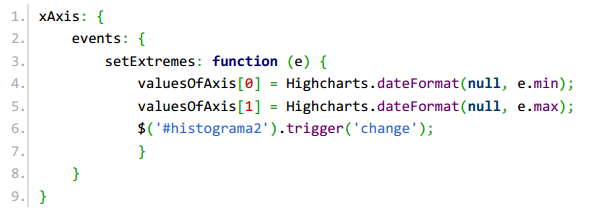
\includegraphics[scale=0.8]{images/onChangeEventTimeline.png}
	\caption[Implementación de evento de detección de cambios en la línea temporal.]{Implementación de evento de detección de cambios en la línea temporal.\\Fuente: Elaboración Propia, (2016)}
	\label{fig:implementacionCambiosEnEje}
\end{figure}

Tras la selección de intervalo dentro del cual se desea que el sistema muestre los estados recibidos, se implementó un servicio REST, donde mediante una consulta del tipo POST con parámetros fecha inicial y final, retornase una lista con todos los marcadores encontrados.

Las categorías mencionadas a continuación son descritas en la sección \ref{sec:diseno:categorias}. Los iconos correspondientes a las categorías que soporta el programa se definieron mediante la combinación de dos imágenes para cada categoría: un marcador de mapa, similar a los definidos en la API de Google Maps y una que sugiriera al usuario el tipo al cual se refiere. Los diseños finales son presentados en las Figuras de la \ref{fig:agua} a la \ref{fig:seguridad}.

\begin{figure}[!htb]
	\minipage{0.32\textwidth}
	\centering
	\captionsetup{justification=centering}
	
\includegraphics[scale=1]{images/categorias/agua.png}
	\caption[Icono categoría agua.]{Icono categoría agua.\\Fuente: Elaboración Propia, (2016)}
	\label{fig:agua}
	\endminipage\hfill
	\minipage{0.32\textwidth}
	\centering
	\captionsetup{justification=centering}
	
\includegraphics[scale=1]{images/categorias/alimento.png}
	\caption[Icono categoría alimento.]{Icono categoría alimento.\\Fuente: Elaboración Propia, (2016)}
	\label{fig:alimento}
	\endminipage\hfill
	\minipage{0.32\textwidth}
	\centering
	\captionsetup{justification=centering}
	
\includegraphics[scale=1]{images/categorias/electricidad.png}
	\caption[Icono categoría electricidad.]{Icono electricidad agua.\\Fuente: Elaboración Propia, (2016)}
	\label{fig:electricidad}
	\endminipage\hfill
\end{figure}

\begin{figure}[!htb]
	\minipage{0.32\textwidth}
	\centering
	\captionsetup{justification=centering}
	
\includegraphics[scale=1]{images/categorias/comunicacion.png}
	\caption[Icono categoría comunicacion.]{Icono categoría comunicacion.\\Fuente: Elaboración Propia, (2016)}
	\label{fig:comunicacion}	
	\endminipage\hfill
	\minipage{0.32\textwidth}
	\centering
	\captionsetup{justification=centering}
	
\includegraphics[scale=1]{images/categorias/personas.png}
	\caption[Icono categoría personas.]{Icono categoría personas.\\Fuente: Elaboración Propia, (2016)}
	\label{fig:personas}
	\endminipage\hfill
	\minipage{0.32\textwidth}
	\centering
	\captionsetup{justification=centering}
	
\includegraphics[scale=1]{images/categorias/seguridad.png}
	\caption[Icono categoría seguridad.]{Icono categoría seguridad.\\Fuente: Elaboración Propia, (2016)}
	\label{fig:seguridad}
	\endminipage\hfill
\end{figure}

Se consideró apropiado, además, diseñar un icono que representara la densidad de marcadores al momento de realizar el agrupamiento por categorías descrito en ésta sección para ello y siguiendo la combinación de colores utilizada por la biblioteca \textit{MarkerClusterer}, \cite{MarkerClusterer}, donde se muestra un cluster azul cuando es un cluster pequeño; amarillo para uno medio y rojo para uno grande. El tamaño de cada uno de estos es especificado internamente por la biblioteca:

\begin{itemize}
\item Azul: De dos a diez elementos.
\item Amarillo: De once a cien elementos amarillo.
\item Rojo: Desde cien elementos.
\end{itemize}

Se prepararon, entonces, tres iconos adicionales a cada categoría para reemplazar los íconos por defecto de la biblioteca, las que pueden verse en las Figuras \ref{fig:aguaS}. a la \ref{fig:seguridadL}.

\begin{figure}[H]
	\minipage{0.32\textwidth}
	\centering
	\captionsetup{justification=centering}
	
\includegraphics[scale=1]{images/categorias/aguaS.png}
	\caption[Icono categoría agua para cluster pequeño.]{Icono categoría agua para cluster pequeño.\\Fuente: Elaboración Propia, (2016)}
	\label{fig:aguaS}
	\endminipage\hfill
	\minipage{0.32\textwidth}
	\centering
	\captionsetup{justification=centering}
	
\includegraphics[scale=1]{images/categorias/aguaM.png}
	\caption[Icono categoría agua para cluster medio.]{Icono categoría agua para cluster medio.\\Fuente: Elaboración Propia, (2016)}
	\label{fig:aguaM}
	\endminipage\hfill
	\minipage{0.32\textwidth}
	\centering
	\captionsetup{justification=centering}
	
\includegraphics[scale=1]{images/categorias/aguaL.png}
	\caption[Icono categoría agua para cluster grande.]{Icono categoría agua para cluster grande.\\Fuente: Elaboración Propia, (2016)}
	\label{fig:aguaL}
	\endminipage\hfill
\end{figure}

\begin{figure}[H]
	\minipage{0.32\textwidth}
	\centering
	\captionsetup{justification=centering}
	
\includegraphics[scale=1]{images/categorias/alimentoS.png}
	\caption[Icono categoría alimento para cluster pequeño.]{Icono categoría alimento para cluster pequeño.\\Fuente: Elaboración Propia, (2016)}
	\label{fig:alimentoS}
	\endminipage\hfill
	\minipage{0.32\textwidth}
	\centering
	\captionsetup{justification=centering}
	
\includegraphics[scale=1]{images/categorias/alimentoM.png}
	\caption[Icono categoría alimento para cluster medio.]{Icono categoría alimento para cluster medio.\\Fuente: Elaboración Propia, (2016)}
	\label{fig:alimentoM}
	\endminipage\hfill
	\minipage{0.32\textwidth}
	\centering
	\captionsetup{justification=centering}
	
\includegraphics[scale=1]{images/categorias/alimentoL.png}
	\caption[Icono categoría alimento para cluster grande.]{Icono categoría alimento para cluster grande.\\Fuente: Elaboración Propia, (2016)}
	\label{fig:alimentoL}
	\endminipage\hfill
\end{figure}

\begin{figure}[H]
	\minipage{0.32\textwidth}
	\centering
	\captionsetup{justification=centering}
	
\includegraphics[scale=1]{images/categorias/electricidadS.png}
	\caption[Icono categoría electricidad para cluster pequeño.]{Icono categoría electricidad para cluster pequeño.\\Fuente: Elaboración Propia, (2016)}
	\label{fig:electricidadS}
	\endminipage\hfill
	\minipage{0.32\textwidth}
	\centering
	\captionsetup{justification=centering}
	
\includegraphics[scale=1]{images/categorias/electricidadM.png}
	\caption[Icono categoría electricidad para cluster medio.]{Icono categoría electricidad para cluster medio.\\Fuente: Elaboración Propia, (2016)}
	\label{fig:electricidadM}
	\endminipage\hfill
	\minipage{0.32\textwidth}
	\centering
	\captionsetup{justification=centering}
	
\includegraphics[scale=1]{images/categorias/electricidadL.png}
	\caption[Icono categoría electricidad para cluster grande.]{Icono categoría electricidad para cluster grande.\\Fuente: Elaboración Propia, (2016)}
	\label{fig:electricidadÑ}
	\endminipage\hfill
\end{figure}

\begin{figure}[H]
	\minipage{0.32\textwidth}
	\centering
	\captionsetup{justification=centering}
	
\includegraphics[scale=1]{images/categorias/comunicacionS.png}
	\caption[Icono categoría comunicación para cluster pequeño.]{Icono categoría comunicación para cluster pequeño.\\Fuente: Elaboración Propia, (2016)}
	\label{fig:comunicacionS}
	\endminipage\hfill
	\minipage{0.32\textwidth}
	\centering
	\captionsetup{justification=centering}
	
\includegraphics[scale=1]{images/categorias/comunicacionM.png}
	\caption[Icono categoría comunicación para cluster medio.]{Icono categoría comunicación para cluster medio.\\Fuente: Elaboración Propia, (2016)}
	\label{fig:comunicacionM}
	\endminipage\hfill
	\minipage{0.32\textwidth}
	\centering
	\captionsetup{justification=centering}
	
\includegraphics[scale=1]{images/categorias/comunicacionL.png}
	\caption[Icono categoría comunicación para cluster grande.]{Icono categoría comunicación para cluster grande.\\Fuente: Elaboración Propia, (2016)}
	\label{fig:comunicacionL}
	\endminipage\hfill
\end{figure}

\begin{figure}[H]
	\minipage{0.32\textwidth}
	\centering
	\captionsetup{justification=centering}
	
\includegraphics[scale=1]{images/categorias/personasS.png}
	\caption[Icono categoría personas para cluster pequeño.]{Icono categoría personas para cluster pequeño.\\Fuente: Elaboración Propia, (2016)}
	\label{fig:personasS}
	\endminipage\hfill
	\minipage{0.32\textwidth}
	\centering
	\captionsetup{justification=centering}
	
\includegraphics[scale=1]{images/categorias/personasM.png}
	\caption[Icono categoría personas para cluster medio.]{Icono categoría personas para cluster medio.\\Fuente: Elaboración Propia, (2016)}
	\label{fig:personasM}
	\endminipage\hfill
	\minipage{0.32\textwidth}
	\centering
	\captionsetup{justification=centering}
	
\includegraphics[scale=1]{images/categorias/personasL.png}
	\caption[Icono categoría personas para cluster grande.]{Icono categoría personas para cluster grande.\\Fuente: Elaboración Propia, (2016)}
	\label{fig:personasL}
	\endminipage\hfill
\end{figure}

\begin{figure}[H]
	\minipage{0.32\textwidth}
	\centering
	\captionsetup{justification=centering}
	
\includegraphics[scale=1]{images/categorias/seguridadS.png}
	\caption[Icono categoría seguridad para cluster pequeño.]{Icono categoría seguridad para cluster pequeño.\\Fuente: Elaboración Propia, (2016)}
	\label{fig:seguridadS}
	\endminipage\hfill
	\minipage{0.32\textwidth}
	\centering
	\captionsetup{justification=centering}
	
\includegraphics[scale=1]{images/categorias/seguridadM.png}
	\caption[Icono categoría seguridad para cluster medio.]{Icono categoría seguridad para cluster medio.\\Fuente: Elaboración Propia, (2016)}
	\label{fig:seguridadM}
	\endminipage\hfill
	\minipage{0.32\textwidth}
	\centering
	\captionsetup{justification=centering}
	
\includegraphics[scale=1]{images/categorias/seguridadL.png}
	\caption[Icono categoría seguridad para cluster grande.]{Icono categoría seguridad para cluster grande.\\Fuente: Elaboración Propia, (2016)}
	\label{fig:seguridadL}
	\endminipage\hfill
\end{figure}

Dado que se solicitó que la interfaz no se recargue cada vez que se produzca un cambio dado por un nuevo evento detectado o el modificación en el intervalo de visualización. Para ello se utilizaron las facultados de Javascript y AJAX capturando los cambios en la línea temporal, descrita en esta sección. Cada vez que se detecte un cambio, se elimina todo marcador del mapa y se reubican en el todos los que cumplan con los parámetros de búsqueda.

\subsubsection*{Estadísticas de procesamiento}
\label{subsubsec:estadisticasdeproc}

Específicamente se solicitaron tres tipos de estadísticas que han de ser mostradas por consulta, estas se definen a continuación:

\begin{enumerate}
\item Cantidad de eventos detectados, es decir, \textit{tweets} que fueron clasificados.
\item Cantidad de usuarios distintos identificados en aquellos eventos.
\item Cantidad total de \textit{tweets} que han pasado por el sistema desde el inicio de la consulta actual.
\end{enumerate}

Para cumplir lo solicitado hacía falta añadir elementos no considerados en la base de datos; hace falta conocer al usuario y contar los \textit{tweets} ingresados desde \textit{Twitter4J}.

Para completar esta historia se realizaron modificaciones al esquema previamente definido en la sección \ref{sec:diseno:persistencia}, este de por si era suficiente para cumplir con la estadística número uno, pero incapaz de realizar las otras dos. Para la segunda estadística se consideró que bastaba con guardar al usuario junto con la colección de marcadores. De acuerdo a \cite{TwitterAgreement} en su sección F. \textit{Be a Good Partner to Twitter}, se insta a los desarrolladores que almacenen contenido \textit{offline} de \textit{Twitter}, a almacenar sólo el ID del usuario o del \textit{tweet}, por ello y siguiendo estos lineamientos se agrega el campo "userID" al esquema marcadores, pasando a quedar como se aprecia en la Figura \ref{fig:esquemaMarker2}.

\begin{figure}[H]
	\centering
	\captionsetup{justification=centering}
	\includegraphics[scale=0.8]{images/Marker2.png}
	\caption[Ejemplo de documento en la colección Markers.]{Ejemplo de documento en la colección Markers.\\Fuente: Elaboración Propia, (2016)}
	\label{fig:esquemaMarker2}
\end{figure}

Para la tercera estadística la colección de marcadores no sería útil, pues no refleja la cantidad de tweets procesados, para ello es necesario implementar una tercera colección de documentos en la base de datos y almacenarlos antes de la aplicación de cualquier tipo de filtro. Esta colección tiene el esquema presente en la Figura \ref{fig:esquemaTweet}.

\begin{figure}[H]
	\centering
	\captionsetup{justification=centering}
	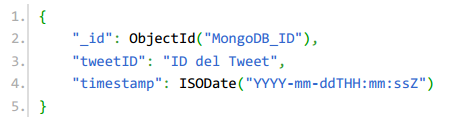
\includegraphics[scale=0.8]{images/status.png}
	\caption[Ejemplo de documento en la colección Status.]{Ejemplo de documento en la colección Status.\\Fuente: Elaboración Propia, (2016)}
	\label{fig:esquemaTweet}
\end{figure}

Al almacenar sólo el contenido del texto no viola las políticas de uso descritas de \textit{Twitter}, sólo es necesario la fecha para la estadística realizar la estadística, pero resulta útil almacenar el contenido para realizar la expansión de la consulta descrita en la sección \ref{subsubsec:2op} y no aumentar la latencia almacenando el ID y realizando una nueva consulta a la API de \textit{Twitter}.

En general la obtención de estas estadísticas se da utilizando el Algoritmo \ref{alg:estadisticas} descrito a continuación.\\

\begin{algorithm}[H]\setstretch{1.5}
	\begin{algorithmic}[numeracion_lineas]
		\REQUIRE Colección $c$ 
		\REQUIRE Fecha de la consulta actual $f$ 
		\ENSURE Contador de eventos $counter$  
		\STATE $counter = 0$
		\FOR{Documento $d_{i}$ en la colección $c$}
			\IF{ fecha de $d_{i}$ es posterior a $f$}
				\STATE $counter = counter + 1$
			\ENDIF	
		\ENDFOR
		\RETURN $counter$
	\end{algorithmic}
	\caption{Algoritmos de generación de primera y tercera estadística.}
	\label{alg:estadisticas}
\end{algorithm}\vphantom\\

Este algoritmo, como se mencionó, es de uso general y permite cumplir tanto la primera como la tercera estadística, para el caso de la segunda se requiere una modificación, pues se solicitó conocer los usuarios diferentes, el algoritmo \ref{alg:estadisticas2} presenta el algoritmo modificado para la segunda estadística.\\

\begin{algorithm}[H]\setstretch{1.5}
	\begin{algorithmic}[numeracion_lineas]
		\REQUIRE Colección $c$ 
		\REQUIRE Fecha de la consulta actual $f$ 
		\ENSURE Lista de usuarios vacía $list$  
		\FOR{Documento $d_{i}$ en la colección $c$}
			\IF{ fecha de $d_{i}$ es posterior a $f$}
				\IF{ID del usuario de $d_{i}$ no está en $list$ o $list$ es vacía}
					\STATE Añadir $d_{i}$ a $list$
				\ENDIF
			\ENDIF	
		\ENDFOR
		\RETURN Cantidad de elementos en $list$
	\end{algorithmic}
	\caption{Algoritmos de generación de segunda estadísticas.}
	\label{alg:estadisticas2}
\end{algorithm}\vphantom\\

Adicionalmente a lo anteriormente descrito hace falta un medio para obtener los datos, para ello se implementó un servicio REST donde utilizando un método GET se obtienen todos los datos correspondientes a la actual consulta activa en el sistema, para conocer cuál fue la última consulta del sistema se utiliza la clase \textit{CurrentQueryChecker}, la cual provee de un método para obtener la fecha de la última consulta.

\subsubsection*{Configuración}
\label{subsubsec:config}

Esta historia nace producto de la HU-v01. El visualizador de eventos tiene dos maneras de comportarse:

\begin{itemize}
\item Modo tiempo real: Cuando el sistema esté en funcionamiento y cada cierto tiempo, $t_{1}$, se actualizan los marcadores de los nuevos eventos y éstos se muestran durante un tiempo, $t_{2}$.
\item Modo línea de tiempo: Funcionamiento basado en lo descrito en HU-v04.
\end{itemize}

Los tiempos $t_{1}$ y $t_{2}$, inicialmente fueron decididos de manera arbitraria, pero al mostrar su funcionamiento se sugirió que estos parámetros fuesen modificados, por ello, se implementó una sección de configuración dentro de la aplicación de visualización para permitir el cambio de estos valores.

\subsection{Detector de necesidades}
\label{subsec:detectorNecesidades}

El detector de necesidades, al estar construido sobre \textit{Apache Storm}, está compuesto de múltiples operadores que trabajan en conjunto.

\subsubsection*{Entrada de datos al sistema}
\label{subsubseC:EntradaDeDatos}

Conociendo desde donde se obtiene la información y teniendo acceso a ella resta conocer cómo realizar la conexión. Para ello se selecciono utilizar \textit{Twitter4J}, una biblioteca no oficial de Java para las API de \textit{Twitter}. Para su funcionamiento sólo requiere del uso de Java en su version 5 o superior.

La implementación de lo anteriormente descrito se realiza utilizando una instancia del objeto \textit{TwitterStream}, el cual captura el flujo público de \textit{Twitter}, almacenando cada estado recibido en una cola. Con esto en mente se construyó el primer operador del sistema correspondiente al \textit{Spout} que surte de datos al sistema.

\begin{figure}[H]
	\centering
	\captionsetup{justification=centering}
	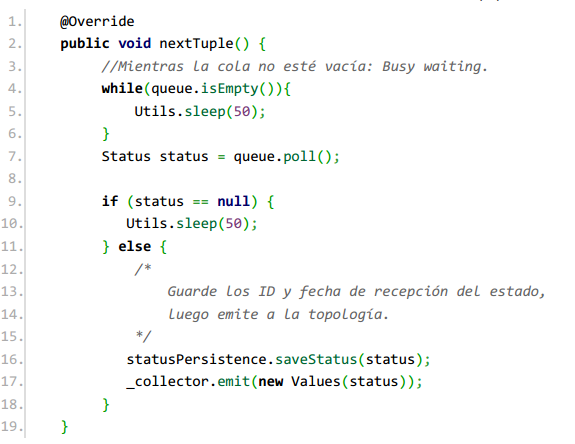
\includegraphics[scale=0.8]{images/TwitterSpout.png}
	\caption[Implementación del \textit{Spout} del sistema.]{Implementación del \textit{Spout} del sistema.\\Fuente: Elaboración Propia, (2016)}
	\label{fig:TwitterSpout}
\end{figure}

Considerando lo recién expuesto la Figura \ref{fig:TwitterSpout} muestra cómo los estados son emitidos por el \textit{spout} al sistema basándose en la cola (\textit{queue}) para manejar lo que llega desde el \textit{stream}

Tal y como se mencionó en el capítulo \ref{cap:MarcTeorico} una topología \textit{storm} funciona estableciendo un grafo donde cada nodo corresponde a un operador o \textit{bolt}, la Figura \ref{fig:stormBeLike} muestra como los \textit{bolt} se unen con el propósito de procesar las entradas entregadas por los \textit{spout} que, en este caso y tal como se señaló en el sección \ref{subsubseC:EntradaDeDatos} corresponde a aquel que recibe la información desde el \textit{stream} de \textit{Twitter}, pero ¿cuál es la función de cada uno de los \textit{bolts}?

La pregunta anteriormente planteada abre un nuevo abanico de problemas, para cada uno de los cuales se desarrolla un operador y éstos, trabajando en conjunto, producen la información necesaria para ser almacenada como un documento 'marcador' en la colección 'Markers' descrita en la Figura \ref{fig:esquemaMarker2}.

\subsubsection*{Operador idioma}
\label{subsubsec:1op}

La primera de las problemáticas a tratar es el idioma. De acuerdo a \cite{TwitterActiveUsers}, existen actualmente 310 millones de usuarios activos en \textit{Twitter} (a enero del 2016), de los cuales 65 millones pertenecen a los Estados Unidos según \cite{TwitterStats1}, y se estima que este año, en latinoamérica, Brasil alcance los 15 millones de usuarios según \cite{TwitterStats2}, sin considerar paises árabes o asiáticos ya se tiene cerca del 30\% de los usuarios activos de \textit{Twitter} hablan, en general, idiomas distintos al Español. Dado que el sistema está pensado para operar dentro de Chile donde el idioma oficial es el Español hace necesario que uno de los operadores, el primero, se el filtrado por idioma, ¿Por qué el primero? Para no realizar procesamiento innecesario con datos que no se han de utilizar.

\cite{languageDetector} desarrolló, haciendo uso de un clasificador \textit{Naïve Bayes}, un módulo escrito en Java el cual es capaz de detectar con éxito 49 idiomas dentro del texto con un 99.8\% de precisión y fue la primera opción para resolver el problema del idioma, pero al analizar el cuerpo de un estado de \textit{Twitter} se encontró que uno de sus campos, precisamente, correspondía al idioma en el que estaba escrito el \textit{tweet}, por ello, y con objeto de no realizar cálculos innecesarios, se optó por utilizar este campo.

La Figura \ref{fig:operadorIdioma} presenta el código de la implementación de este \textit{bolt}, correspondiente a su método \textit{execute}, descrito en la sección \ref{subsec:HerrDesarrollo}.

\begin{figure}[H]
	\centering
	\captionsetup{justification=centering}
	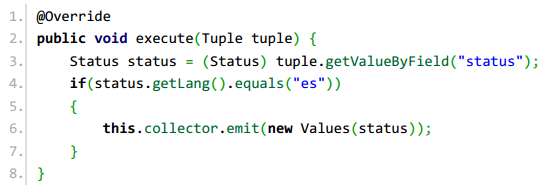
\includegraphics[scale=0.8]{images/LanguageBoltExecute.png}
	\caption[Implementación del método \textit{execute} del \textit{bolt} de idioma.]{Implementación del método \textit{execute} del \textit{bolt} de idioma.\\Fuente: Elaboración Propia, (2016)}
	\label{fig:operadorIdioma}
\end{figure}

Aunque simple, éste operador filtra un gran número de estados, dado que según lo dicho anteriormente, la mayoría de los usuarios de \textit{Twitter} no son hispano-hablantes. 

\subsubsection*{Operador filtro de consultas}
\label{subsubsec:2op}

El segundo problema corresponde a que aunque se tengan los mensajes en el idioma correcto existen mensajes que el usuario desea que sean priorizados, para ello, y como se definió en la sección \ref{sec:diseno:termBusqueda}, son entregados términos de búsqueda. Es así como el segundo nivel de operadores corresponda a aplicar los filtros de búsqueda ingresados por el usuario, si existiesen, aplicando el algoritmo descrito anteriormente y discriminando aquellos estados que contengan las palabras buscadas.

Adicionalmente, la historia HU-c02 que guarda relación con la HU-v05, menciona la necesidad de incrementar los términos de búsqueda para enriquecerla y abarcar la mayor información posible dado una consulta. Para realizar esto se consideró una práctica del procesamiento de lenguaje natural como es la denominada \textit{Query Expansion} (QE). Según lo descrito por \cite{IRQE} son técnicas comunes al utilizar QE la búsqueda de sinónimos (uso de diccionarios priviamente establecidos), diccionarios basados en la minería de los elementos previamente hayados, creación de diccionadios basados en la co-ocurrencia de términos, es decir, términos que suelen venir juntos o un vocabulario mantenido por editores humanos. Para este trabajo sólo se consideran las dos primeras: Búsqueda por diccionario de sinónimos y una implementación que encuentra los términos más frecuentes dentro de los resultados de la búsqueda.

El diccionario de sinónimos es básicamente una bolsa de palabras asociadas a una semilla, es decir, dado un término de búsqueda agregar todos los términos asociados a el en el diccionario.

En el caso de la búsqueda de términos frecuentes se sugirió integrar un proyecto \textit{storm} ya desarrollado el cuál tiene por finalidad la búsqueda de los denominados \textit{thrending topics}, es decir, aquellos términos de los que se realizan más menciones en un determinado instante, pero aquella implementación sólo consideraba los denominados \textit{hashtag}, un marcador de palabras concatenadas que inician por el caracter "\#". Siendo ese el caso el uso de esta topología storm no es del todo util. En su lugar se desarrolla un contador de frecuencias para palabras con un funcionamiento similar, dicha implementación se aprecia en el Algoritmo \ref{alg:TT}.\\

\begin{algorithm}[H]\setstretch{1.5}
	\begin{algorithmic}[numeracion_lineas]
		\REQUIRE Estados $E=\{e_{1}, \dots, e_{n} \}$.
		\ENSURE Terminos frecuentados $T=\{t_{1}, \dots, t_{10} \}$.
		\STATE Lista de terminos: $l$.
		\FOR{Estado: $e_{i}$}
			\STATE Dividir estado por palabra.
			\STATE Eliminar \textit{stopword} de las palabras.
			\FOR{Palabra: $w_{i}$ en $e_{i}$}
				\IF{ $w_{i}$ está en  $l_{i}$}
					\STATE aumentar contador de $w_{i}$ en $l_{i}$.
				\ELSE
					\STATE agregar $w_{i}$ a $l_{i}$ con contador en 1.
				\ENDIF		
			\ENDFOR
		\ENDFOR
		\IF{$l_{i}$ tiene menos de 10 elementos}
			\RETURN $l_{i}$
		\ELSE
			\RETURN los 10 primeros elementos de $l_{i}$.
		\ENDIF
	\end{algorithmic}
	\caption{Algoritmos de términos recurrentes.}
	\label{alg:TT}
\end{algorithm}\vphantom\\

Dado que el operador puede estar replicado no se reciben los mismos estados a todas las instancias del nodo, por ello este proceso se realiza de manera única para cada instancia en función de los estados que hayan llegado a él. El Algoritmo \ref{alg:TT} agrega a los términos de búsqueda de cada instancia las palabras más frecuentes y, siguiendo el ejemplo de \textit{Twitter} con sus \textit{thrending topics} tiene un máximo de diez nuevas palabras.

\begin{figure}[H]
	\centering
	\captionsetup{justification=centering}
	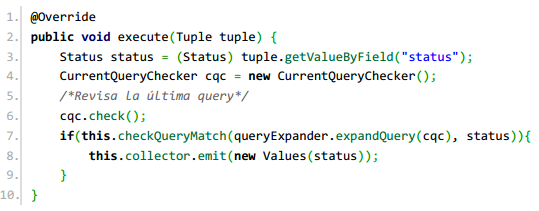
\includegraphics[scale=0.8]{images/FilterBolt.png}
	\caption[Implementación del método \textit{execute} del \textit{bolt} del filtro de consultas.]{Implementación del método \textit{execute} del \textit{bolt} del filtro de consultas.\\Fuente: Elaboración Propia, (2016)}
	\label{fig:operadorFiltro}
\end{figure}

La Figura \ref{fig:operadorFiltro} muestra la implementación del filtro de consultas. Hace uso de instancias de los objetos descritos en HU-v05 para encontrar la última consulta en el sistema y expande la consulta según ésta y los resultados obtenidos en los estados recibidos. Finalmente y si el estado contiene algunos los términos especificados, éste es emitido al siguiente nivel de operadores.

\subsubsection*{Operador normalizador de texto}
\label{subsubsec:3op}

El tercer problema es inherente a \textit{Twitter}: En esta red social es común referenciar un estado a un determinado tema, he ahí el uso de los conocidos \textit{Hashtag} que, como se mencionó en la sección \ref{subsubsec:estadisticasdeproc} corresponden a palabras concatenadas antecedidas por el caracter \#. Otro problema común corresponde a la mención de usuarios, ésta corresponde a un llamado al nombre de usuario dentro de la aplicación, antecedida por el caracter "@", usualmente usada para el envío de mensajes entre pares. Diversos autores, entre ellos, \cite{NLPaccuracy}, \cite{NLPaccuracy1} y \cite{NLPaccuracy2}, han señalado que la existencia de estos elementos significan una disminución en la precisión de los elementos descritos en la sección \ref{sec:diseno:clasificador}. Por ello él tercer operador corresponde a normalizador de texto, el cual reemplaza menciones a usuarios, \textit{hashtags} y URLs, todas ellas variables, por palabras constantes, el reemplazo a realizarse se muestra en la Tabla \ref{tab:reemplazosDeEntidades}.

\begin{table}[H]
\centering
\caption[Reemplazo de entidades en texto.]{Reemplazo de entidades en texto.\\Fuente: Elaboración Propia, (2016)}
\label{tab:reemplazosDeEntidades}
\begin{tabular}{|c|c|}
\hline
\textbf{Entidad} & \textbf{Reemplazo} \\ \hline
@usuario         & USUARIO            \\ \hline
\#hashtag        & HASHTAG            \\ \hline
http://var.foo/  & URL                \\ \hline
\end{tabular}
\end{table}

La implementación de éste operador se realizo utilizando expresiones regulares para detectar cuándo se está haciendo referencia a uno de los elementos anteriores y luego aplicar su reemplazo.

\subsubsection*{Operador geolocalizador}
\label{subsubsec:4op}

El cuarto y mayor problema presentado tiene relación, principalmente, con la historia HU-v01. Si bien se mencionó cómo se realiza la visualización, no se señaló cómo es que se obtienen tanto la coordenadas geográficas, latitud y longitud, para ubicar geográficamente un evento.

Ha sido señalado por \cite{ChatoSurvey} que menos del 1\% de los \textit{tweets} contienen datos en sus campos correspondientes a geolocalización. En un experimento (véase Apéndice \ref{apendice:apendice1}) realizado utilizando la herramienta \textit{RapidMiner} se obtuvo una muestra de 67.789 \textit{tweets} directamente desde el \textit{stream} sin utilizar filtros de búsqueda, de esos \textit{tweets} 67.475 no contaban con los datos correspondientes a la ubicación geográfica, es decir, el 0.46\% de los datos de aquella muestra cuentan con la información requerida, lo que hace creer que lo presentado por los autores, antes mencionados, está en lo correcto.

Siendo la geolocalización un elemento de suma importancia para el funcionamiento de la aplicación, se ha de intentar obtener este dato de alguna forma. Así es como surge la posibilidad de usar el contenido del \textit{tweet} para obtener la ubicación, para ello se preparó un diccionario con las comunas del país y sus coordenadas geográficas, \cite{ubicacionesChile} y se diseñó el Algoritmo \ref{alg:geolocalizacion}. De esta manera existe una aproximación para detectar la ubicación a la que un \textit{tweet} hace referencia.\\

\begin{algorithm}[H]\setstretch{1.5}
	\begin{algorithmic}[numeracion_lineas]
		\REQUIRE Lista de ciudades $C=\{c_{1}, \dots, c_{n} \}$.
		\REQUIRE Tweet $t$.
		\ENSURE Coordenadas geográficas $P=\{latitud, longitud\}$.
		\IF{$t$ está geolocalizado}
			\IF{Está dentro del territorio chileno}
				\RETURN Coordenadas del $t$.
			\ELSE
				\RETURN Fuera de Chile.
			\ENDIF
		\ELSE
			\IF{El texto de $t$ contiene elementos presentes en $C$}
				\RETURN Coordenadas de $c_{i}$.
			\ELSE
				\RETURN No geolocalizable.
			\ENDIF
		\ENDIF
	\end{algorithmic}
	\caption{Algoritmos de ubicación geoográfica.}
	\label{alg:geolocalizacion}
\end{algorithm}\vphantom\\

Para detectar cuándo una ubicación está en Chile, se generó un cuadro en el mapa donde se delimita todo el territorio Chileno, incluyendo Isla de Pascua.

Haciendo uso del algoritmo desarrollado es posible aumentar la cantidad de elementos que continúan en la línea de procesamiento. En el capítulo \ref{cap:experimentos} realiza una evaluación sobre la efectividad del operador.

Los operadores descritos en las secciones \ref{subsubsec:5op} y \ref{subsubsec:6op} tienen relación con la labor del señalado en \ref{subsubsec:7op}, las razones que llevan a la construcción de estos tres son expuestan en la sección \ref{subsubsec:clasificacion}, mientras tanto, al igual que los operadores anteriores se detalla el cómo fueron diseñados.

\subsubsection*{Operador removedor de \textit{stopword}}
\label{subsubsec:5op}

Éste operador hace uso de una lista de palabras denominadas \textit{stopwords} o palabras vacías, éstas corresponden a palabras sin significado, como artículos, pronombres, preposiciones, etcétera. Éstas palabras son eliminadas del texto que se está procesando, para ello se utiliza el Algoritmo \ref{alg:stopwords}.\\

\begin{algorithm}[H]\setstretch{1.5}
	\begin{algorithmic}[numeracion_lineas]
		\REQUIRE Lista de \textit{stopwords} $S=\{s_{1}, \dots, s_{n} \}$.
		\REQUIRE Texto $T$.
		\ENSURE Texto $T'$.
		\STATE $T'$ = $T$
		\FOR{cada palabra de $T$, $t_{i}$}
			\IF{$t_{i}$ está contenida en $S$}
			\STATE $T'$ = $T'$ - $t_{i}$. 
			\ENDIF
		\ENDFOR
		\RETURN $T'$
	\end{algorithmic}
	\caption{Algoritmos de eliminiación de \textit{stopwords}.}
	\label{alg:stopwords}
\end{algorithm}\vphantom\\

\subsubsection*{Operador raíz de texto}
\label{subsubsec:6op}

Este operador hace uso del algoritmo de \cite{Porter}, para extraer prefijos y sufijos de palabras y llevarlas a una raíz común, \cite{StemmingLema}, son ejemplos de este proceso, denominada \textit{stemming}, las palabras presentadas en la Tabla \ref{tab:ejstemming}

\begin{table}[H]
\centering
\caption[Ejemplo de \textit{stemming} para la palabra 'presentar'.]{Ejemplo de \textit{stemming} para la palabra 'presentar'.\\Fuente: Elaboración Propia, (2016)}
\label{tab:ejstemming}
\begin{tabular}{|c|c|}
\hline
\textbf{Palabra} & \textbf{Combinaciones de Sufijos} \\ \hline
Presentarla      & arla                              \\ \hline
Presentarlas     & arlas                             \\ \hline
Presentarle      & arle                              \\ \hline
Presentarles     & arles                             \\ \hline
Presentarlo      & arlo                              \\ \hline
Presentarlos     & arlos                             \\ \hline
Presentarse      & arse                              \\ \hline
Presentase       & ase                               \\ \hline
Presentásemos    & ásemos                            \\ \hline
Presente         & e                                 \\ \hline
Presentémonos    & émonos                            \\ \hline
\end{tabular}
\end{table}

\subsubsection*{Operador etiquetador}
\label{subsubsec:7op}

Este operador hace uso del clasificador generado mediante las técnicas descritas en la sección \ref{sec:diseno:categorias}, para etiquetar el texto de acuerdo a la categoría a la que corresponda. Una vez realizado este proceso se cuenta con todos los datos necesarios para generar completamente un documento de la colección 'Markers', presentada en la Figura \ref{fig:esquemaMarker2}.

\subsubsection*{Operador persistencia}
\label{subsubsec:8op}

Este operador se encarga de conectarse a la base de datos y almacenar el nuevo marcador. Los datos recibidos desde la cadena de procesamiento se lleva a una instancia de objeto Java, llamado "Marker", el cual contiene los mismos elementos descritos para un documento de la colección "Markers", a un objeto JSON utilizando \textit{Jackson} y finalmente, utilizando \textit{Jongo}, lo transforma en BSON para almacenarlo en la base de datos en MongoDB.

\subsubsection*{Construcción del clasificador}
\label{subsubsec:clasificacion}

Hasta ahora se han tocado, prácticamente, todos los temas que se relacionan con el funcionamiento del sistema de detección, desde donde se obtienen los datos, cómo se procesan e incluso cómo se almacenan, pero no se ha especificado cómo se realiza la clasificación, es decir, cómo dado un texto de entrada se consigue discriminar en qué categoría encaja. Ésta sección especifica lo que se contextualizó en la sección \ref{subsubsec:7op}.

El concepto que involucra la construcción de un clasificador es el de "aprendizaje supervizado", que fue mencionado en la sección \ref{subsec:MineriaTexto}, en este tipo de aprendizaje se requiere de un conjunto de datos de entrada, denominados conjunto de entrenamiento, que ha de pasar por el algoritmo, en este caso \textit{Naïve Bayes}, que ha de conocer previamente, la salida esperada para cada elemento del conjunto. El resultado esperado es un clasificador capaz de predecir, en este caso, a qué categoría pertenece un texto sometido a su evaluación.

Según la metodología KDD existen subprocesos en la búsqueda de conocimiento en bases de datos, estos fueron descritos en la sección \ref{subsec:MetodologiaDetalle}, para este caso particular se describe cómo fue realizado cada uno de estos subprocesos para la construcción del clasificador con el que cuenta el sistema.

El subproceso de selección de datos se llevó a cabo extrayendo un subconjunto del \textit{dataset} mencionado en la sección \ref{subsec:alcances}. Éste conjunto, de exactamente 2234 \textit{tweets} correspondientes al del terremoto de Concepción el año 2010, todos ellos en español, pero no todos hacen referencia al evento, pues éste coincidió con la realización de la LI versión del Festival Internacional de la Canción de Viña del Mar y muchos de estos \textit{tweets} hacen referencia a este último. Los datos en este punto de proceso cuentan con los campos correspondientes a un \textit{tweet} de la época, es decir: "ID\_unit", "day", "date", "time\_zone", "time", "tweet\_it", "user\_id", "name", "screen\_name", "friends\_count", "follower\_count", "text" y "value". Todos ellos separados por coma (,).

En cuanto al subproceso de preprocesamiento de datos, el primer paso corresponde a la limpieza de los datos, en conjunto de datos que se está utilizando contenía elementos incompletos que no presentaban texto, estos fueron eliminados, pues no resultaban útiles sin el componente texto, quedando así un total de 2187 \textit{tweets} con datos útiles.

El siguiente paso, correspondiente al suproceso de transformación de datos, del conjunto de datos útiles se extrajo el texto y se eliminaron todos los demás componentes. Llegados a este punto sólo se contaba con una lista de textos de \textit{tweets} en español. Lo siguiente a realizar corresponde al proceso de etiquetado, para ello se leyó cada texto y según su contenido se ubicó en alguna de las categorías descritas en la sección \ref{sec:diseno:categorias}, además se asignó un identificador a cada texto, basado en su número, para ser ingresados a la herramienta Mallet, encargada de la construcción del clasificador, así se obtuvo un archivo con los datos formateados según lo descrito en la sección \ref{sec:diseno:clasificador}, es decir, con los campos "Identificador", "Etiqueta", "Contenido". En este punto los datos fueron ingresados al sistema para la aplicación de los operadores descritos en la sección \ref{subsec:detectorNecesidades}, en particular la eliminación de \textit{stopwords}, normalización de texto y \textit{stemming}.

El cuarto subproceso es automatizado por Mallet y corresponde al minado de datos en sí, para entregarle los datos a Mallet primero han de construirse como un objeto "\textit{Instance}", lo cual se realiza entregándole cada uno de los elementos preparados en la sección anterior: el identificador, etiqueta y contenido que ya ha pasado por las operaciones que componene el subproceso de transformación. Como resultado de este proceso se obtiene un objeto \textit{Classifier}, el cual puede ser serializado y almacenado como un archivo denominado, en este caso, "classifier.dene". 

Finalmente el subproceso de evaluación también es llevado a cabo por la herramienta Mallet, que implementa un objeto denominado "\textit{Trial}" el cual, utilizando un clasificador y un conjunto de datos de prueba. Como resultado de este subproceso se obtienen las métricas comunes de evaluación: \textit{accuracy}, \textit{recall} y \textit{F-1 score}. La evaluación del clasificador construido se presenta en la sección \ref{sec:EvalClassificador} del Capítulo \ref{sec:EvalClassificador}. 

\subsubsection*{Topología del sistema}
\label{subsubsec:topologiaSistema}

Habiendo definido los elementos de procesamiento, los operadores o \textit{bolts}, se está en condicion de definir la topología. La topología que utiliza el sistema, en términos generales de la aplicación está definida en la Figura \ref{fig:TopologiaGeneral}.

La razón de este orden en la topología se debe a varias razones y se justifican a continuación:

\begin{itemize}
\item \textit{Spout Twitter}: Es el eslabón principal de la cadena. Desde aquí se emiten los nuevos estados al sistema y todo el sistema depende de el. 
\item \textit{Bolt} Filtro de idioma: Ocupa la primera posición de los operadores del sistema, dado que se espera que el \textit{stream} reciba estados de todo el mundo y no sólo en español. Al estar este operador en primer lugar se asegura de reducir el flujo en gran medida, lo cual puede comprobarse por los resultados obtenidos en el Capítulo \ref{cap:experimentos}.
\item \textit{Bolt} Filtro de consulta: Habiendo filtrado sólo aquellos estados cuyo lenguage sea el español es necesario filtrar aun más el \textit{stream} valiéndose de las restricciones especificadas por el usuario. Así sólo los estados que contengan términos especificados por el usuario, o el sistema de expansión, continúan en el sistema.
\item\textit{Bolt} Normalizador de texto: Previo al detector de ubicación para evitar posibles confusiones que pueda acarrear la existencia de nombres de lugares en elementos como nombres de usuario, \textit{hashtags} o enlaces.
\item\textit{Bolt} Detección de ubicación: Ocupa ésta posición, pues debe ir previo a la eliminación de \textit{stopwords}, de lo contrario ubicaciones, como por ejemplo "los vilos", válida dentro de chile, es ignorada por el sistema.
\item\textit{Bolt} Eliminador de \textit{stopword}: Se realiza previo al \textit{Stemming} para reducir la carga computacional, pues el operador de \textit{stemming} lleva a palabras raíz estos términos que no son necesarios.
\item\textit{Bolt} \textit{Stemmer}: Es la única ubicación posible para este operador, pues el siguiente paso es etiquetar el estado.
\item\textit{Bolt} Etiquetador: Aplica el modelo al estado, el estado ha de tener su correspondiente etiqueta antes de ser almacenado.
\item\textit{Bolt} Persistencia: último eslabón de la cadena. Ingresa un nuevo documento a la colección de marcadores.
\end{itemize}

\begin{figure}[H]
	\centering
	\captionsetup{justification=centering}
	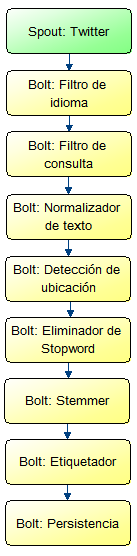
\includegraphics[scale=0.8]{images/TopologiaGeneral.png}
	\caption[Topología general del sistema.]{Topología general del sistema.\\Fuente: Elaboración Propia, (2016)}
	\label{fig:TopologiaGeneral}
\end{figure}





